
\documentclass[tikz,border=10pt]{standalone}
%\documentclass[crop, tikz]{standalone}

\usepackage{tikz}
% needed for Mindmap
\usetikzlibrary{mindmap}

\pgfdeclarelayer{background}
\pgfsetlayers{background,main}

\begin{document}
	

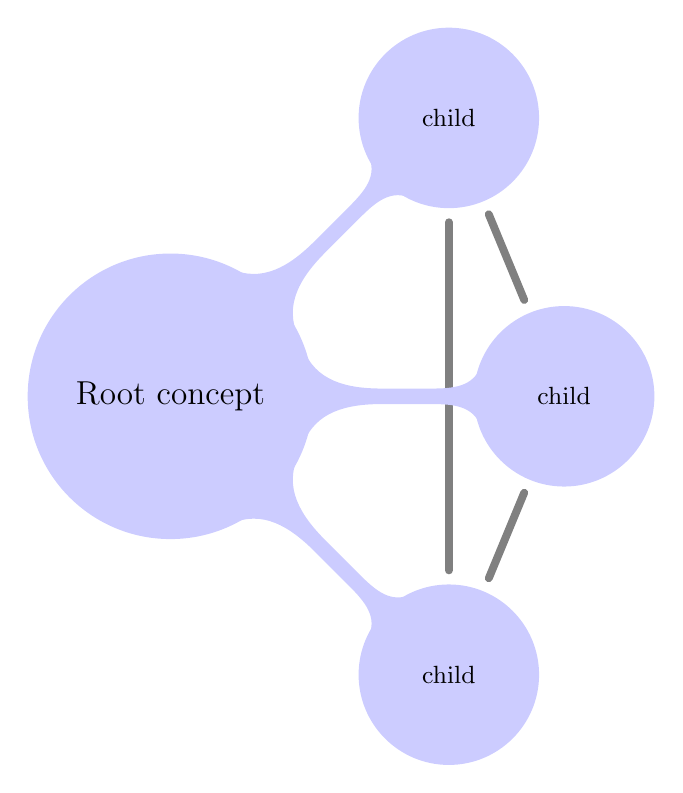
\begin{tikzpicture}
	[root concept/.append style={concept color=blue!20,minimum size=2cm},
	level 1 concept/.append style={sibling angle=45},
	mindmap]
	\node [concept] {Root concept}
	[clockwise from=45]
	child { node[concept] (c1) {child}}
	child { node[concept] (c2) {child}}
	child { node[concept] (c3) {child}};
	\begin{pgfonlayer}{background}
	\draw [concept connection] (c1) edge (c2)
	edge (c3)
	(c2) edge (c3);
	\end{pgfonlayer}
\end{tikzpicture}

	
\end{document}
